\documentclass{article}
\usepackage{graphicx}
\graphicspath{{./Pictures/}}
\usepackage[table,xcdraw]{xcolor}

\title{My first chapter}
\author{Krzysztof Ferda}
\date{3.11.2022}

\begin{document}

\maketitle

\section {Paragraf Krzysztofa Ferdy}
Czym jest liczba \textbf{"e"} w matematyce ?
\\
Liczba \textbf{"e"} jest podstawą logarytmu naturalnego. Nazywa się ją liczbą \textbf{Eulera}. Jest ona wykorzystywana w wielu dziedzinach matematyki i fizyki. Wynosi w przybliżeniu:\underline{2,7182818284.}
\\
\\
\textbf{Jest ona określana przez granicę następującego ciągu:}
    \begin{equation} \label{eq:1}
        \lim_{n \to \infty }\left({1+\frac{1}{n}}\right)^n=e
    \end{equation}
\textbf{Przy rozwiązywaniu zadań może nam się przydać następujący wzór:}
    \begin{equation} \label{eq:2}
        \lim_{n \to \infty }\left({1+\frac{a}{n}}\right)^n=e^a
    \end{equation}
\\
\\
\subsection{Formatowanie numerowane i nienumerowane}

\textbf{Lista nienumerowana:}
\begin{itemize}
  \item Numer jeden
  \item Numer dwa
  \item Numer trzy
\end{itemize}

\textbf{Lista numerowana:}
\begin{enumerate}
    \item jeden 
    \item dwa
    \item trzy
\end{enumerate}
\\
\\
\\
\\
\\
\subsection{Zdjęcie}
\begin{figure}[htbp]
    \centering
    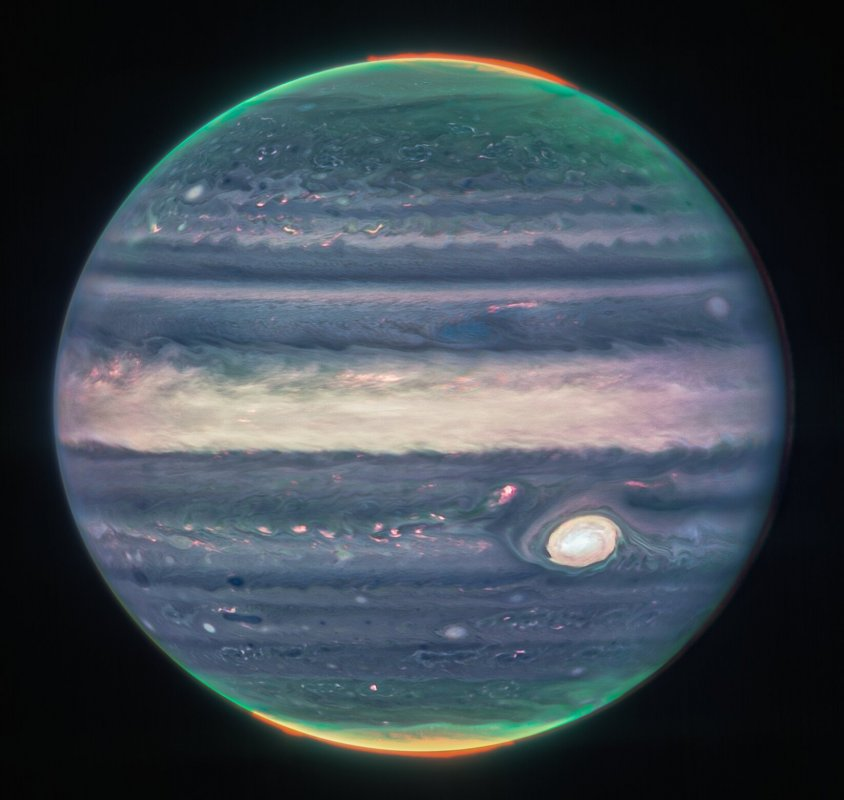
\includegraphics[width=\linewidth]{Pictures/JOWISZ.jpg}
    \caption{Jowisz}
    \label{fig:my_label}
\end{figure}
\\
\subsection{Formatowanie tekstu}
\textbf{Lorem ipsum} \textit{dolor sit amet, consectetur adipiscing elit, sed do eiusmod tempor incididunt ut labore et dolore magna aliqua. Ut enim ad minim veniam, quis nostrud exercitation ullamco laboris nisi ut aliquip ex ea commodo consequat.}
\par \textbf{Lorem ipsum} \textit{dolor sit amet, consectetur adipiscing elit, sed do eiusmod tempor incididunt ut labore et dolore magna aliqua. Ut enim ad minim veniam, quis nostrud exercitation ullamco laboris nisi ut aliquip ex ea commodo consequat.}
\\
\\
\begin{table}[]
\begin{tabular}{l|
>{\columncolor[HTML]{FFFFFF}}c |
>{\columncolor[HTML]{FFFFFF}}c |
>{\columncolor[HTML]{FFFFFF}}c |}
\cline{2-4}
& \multicolumn{1}{l|}{\cellcolor[HTML]{00D2CB}kolumna 1} & \multicolumn{1}{l|}{\cellcolor[HTML]{00D2CB}kolumna 2} & \multicolumn{1}{l|}{\cellcolor[HTML]{00D2CB}kolumna 3} \\ \hline
\multicolumn{1}{|l|}{\cellcolor[HTML]{DAE8FC}*}   & 1 & 1 & 1 \\ \hline
\multicolumn{1}{|l|}{\cellcolor[HTML]{DAE8FC}**}  & 1 & 2 & 2 \\ \hline
\multicolumn{1}{|l|}{\cellcolor[HTML]{DAE8FC}***} & 1 & 2 & 3 \\ \hline
\end{tabular}
\end{table}

\end{document}